\documentclass[aspectratio=169]{beamer}
\usepackage{tikz}
\usepackage{array}
\usepackage{enumitem}
\usepackage{xcolor}
\usepackage{amsmath}
\usepackage{tcolorbox}
\usetikzlibrary{automata,positioning,arrows.meta,backgrounds}
\usetikzlibrary{arrows.meta,positioning,calc,matrix}

% Define colors
\definecolor{myblue}{RGB}{0,0,255}
\definecolor{mypurple}{RGB}{128,0,128}
\definecolor{mygreen}{RGB}{0,128,0}
\definecolor{myorange}{RGB}{255,140,0}
\definecolor{lightblue}{RGB}{173,216,230}
\definecolor{peach}{RGB}{255,218,185}
\definecolor{lightpurple}{RGB}{230,230,250}

\usetheme{default}
\setbeamertemplate{navigation symbols}{}

\begin{document}

% First Slide - Branches and Performance
\begin{frame}
\frametitle{Branches and Performance}
\label{frame:branches_performance}

\begin{itemize}
    \item[$\diamond$] \textbf{Misprediction Rate (MPR) vs. Misprediction Per Instruction (MPI)}
\end{itemize}

\vspace{0.3cm}

\begin{center}
\begin{tabular}{ccc}
$\text{MPR} = \dfrac{\text{\# mis-predicted jumps}}{\text{total \# jump}}$ & \hspace{1cm} & $\text{MPI} = \dfrac{\text{\# mis-predicted jumps}}{\text{total \# instructions}}$
\end{tabular}
\end{center}

\vspace{0.3cm}

\begin{itemize}
    \item[$\triangleright$] MPI correlates better with performance since it takes into account jumps frequency
\end{itemize}

\vspace{0.2cm}

\begin{itemize}
    \item[$\diamond$] \textbf{Assume}
    \begin{itemize}
        \item[$\triangleright$] MPI = 1\% (1 flush every 100 instructions on average)
        \item[$\triangleright$] IPC=2 \hspace{0.5cm} (2 instructions per cycle on average)
        \item[$\triangleright$] Flush penalty of 10 cycles
    \end{itemize}
\end{itemize}

\vspace{0.2cm}

\begin{itemize}
    \item[$\diamond$] \textbf{We get:}
    \begin{itemize}
        \item[$\triangleright$] MPI = 1\% $\Rightarrow$ 1 flush every 100 instructions on average
        \item[$\triangleright$] IPC=2 $\Rightarrow$ 1 flush every 50 cycles
        \item[$\triangleright$] 10 cycles flush penalty every 50 cycles
        \item[$\triangleright$] 20\% in performance
    \end{itemize}
\end{itemize}

\end{frame}

\begin{frame}
\frametitle{What/Who/When We Predict/Fix/Allocate}
\label{frame:predict_fix_allocate}

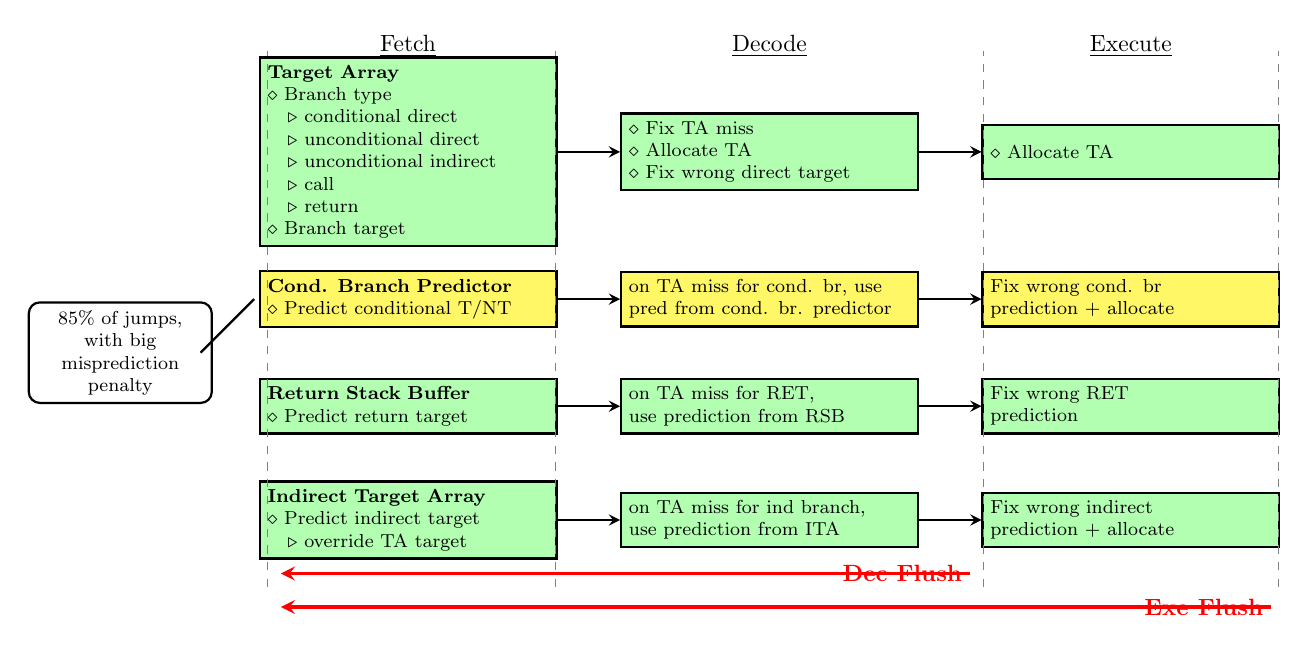
\begin{tikzpicture}[scale=0.85, transform shape,
    box/.style={rectangle, draw=black, thick, minimum height=0.8cm, text width=4.2cm, align=left, font=\footnotesize},
    greenbox/.style={box, fill=green!30},
    yellowbox/.style={box, fill=yellow!60},
    arrow/.style={->, thick, >=stealth}
]

% Column headers
\node[font=\normalsize, anchor=south] at (2.1, 5.8) {\underline{Fetch}};
\node[font=\normalsize, anchor=south] at (7.5, 5.8) {\underline{Decode}};
\node[font=\normalsize, anchor=south] at (12.9, 5.8) {\underline{Execute}};

% Fetch column
\node[greenbox] (ta) at (2.1, 4.5) {
    \textbf{Target Array}\\
    $\diamond$ Branch type\\
    \hspace{0.3cm}$\triangleright$ conditional direct\\
    \hspace{0.3cm}$\triangleright$ unconditional direct\\
    \hspace{0.3cm}$\triangleright$ unconditional indirect\\
    \hspace{0.3cm}$\triangleright$ call\\
    \hspace{0.3cm}$\triangleright$ return\\
    $\diamond$ Branch target
};

\node[yellowbox] (cbp) at (2.1, 2.3) {
    \textbf{Cond. Branch Predictor}\\
    $\diamond$ Predict conditional T/NT
};

\node[greenbox] (rsb) at (2.1, 0.7) {
    \textbf{Return Stack Buffer}\\
    $\diamond$ Predict return target
};

\node[greenbox] (ita) at (2.1, -1.0) {
    \textbf{Indirect Target Array}\\
    $\diamond$ Predict indirect target\\
    \hspace{0.3cm}$\triangleright$ override TA target
};

% Decode column
\node[greenbox] (dec1) at (7.5, 4.5) {
    $\diamond$ Fix TA miss\\
    $\diamond$ Allocate TA\\
    $\diamond$ Fix wrong direct target
};

\node[yellowbox] (dec2) at (7.5, 2.3) {
    on TA miss for cond. br, use\\
    pred from cond. br. predictor
};

\node[greenbox] (dec3) at (7.5, 0.7) {
    on TA miss for RET,\\
    use prediction from RSB
};

\node[greenbox] (dec4) at (7.5, -1.0) {
    on TA miss for ind branch,\\
    use prediction from ITA
};

% Execute column
\node[greenbox] (exe1) at (12.9, 4.5) {
    $\diamond$ Allocate TA
};

\node[yellowbox] (exe2) at (12.9, 2.3) {
    Fix wrong cond. br\\
    prediction + allocate
};

\node[greenbox] (exe3) at (12.9, 0.7) {
    Fix wrong RET\\
    prediction
};

\node[greenbox] (exe4) at (12.9, -1.0) {
    Fix wrong indirect\\
    prediction + allocate
};

% Arrows between columns
\draw[arrow] (ta.east) -- (dec1.west);
\draw[arrow] (cbp.east) -- (dec2.west);
\draw[arrow] (rsb.east) -- (dec3.west);
\draw[arrow] (ita.east) -- (dec4.west);

\draw[arrow] (dec1.east) -- (exe1.west);
\draw[arrow] (dec2.east) -- (exe2.west);
\draw[arrow] (dec3.east) -- (exe3.west);
\draw[arrow] (dec4.east) -- (exe4.west);

% Vertical dashed lines
\draw[dashed, gray] (0, -2) -- (0, 6);
\draw[dashed, gray] (4.3, -2) -- (4.3, 6);
\draw[dashed, gray] (10.7, -2) -- (10.7, 6);
\draw[dashed, gray] (15.1, -2) -- (15.1, 6);

% Left annotation
\node[draw, rounded corners, thick, text width=2.5cm, align=center, font=\footnotesize] at (-2.2, 1.5) {
    85\% of jumps,\\
    with big\\
    misprediction\\
    penalty
};
\draw[thick] (-1.0, 1.5) -- (-0.2, 2.3);

% Red flush arrows
\draw[arrow, red, very thick] (10.5, -1.8) -- (0.2, -1.8);
\node[red, font=\normalsize, anchor=east] at (10.5, -1.8) {\textbf{Dec Flush}};

\draw[arrow, red, very thick] (15, -2.3) -- (0.2, -2.3);
\node[red, font=\normalsize, anchor=east] at (15, -2.3) {\textbf{Exe Flush}};

\end{tikzpicture}

\end{frame}

% Third Slide - The Target Array
\begin{frame}
\frametitle{The Target Array}
\label{frame:target_array}

\begin{columns}[T]
\begin{column}{0.58\textwidth}
\begin{itemize}
    \item[$\diamond$] \textbf{The TA is accessed using the branch address (branch IP)}
    \begin{itemize}
        \item[$\triangleright$] Implemented as an $n$-way set associative cache
    \end{itemize}
\end{itemize}

\vspace{0.15cm}

\begin{itemize}
    \item[$\diamond$] \textbf{The TA predicts the following}
    \begin{itemize}
        \item[$\triangleright$] Instruction is a branch
        \item[$\triangleright$] Predicted target
        \item[$\triangleright$] Branch type
        \begin{itemize}
            \item[$\circ$] Conditional: jump to target if predict taken
            \item[$\circ$] Unconditional direct: take target
            \item[$\circ$] Unconditional Indirect: if ITA hits, use its target
            \item[$\circ$] Return: get target from Return Stack Buffer
        \end{itemize}
    \end{itemize}
\end{itemize}

\vspace{0.15cm}

\begin{itemize}
    \item[$\diamond$] \textbf{The TA is allocated/updated at Decode / EXE}
\end{itemize}

\vspace{0.15cm}

\begin{itemize}
    \item[$\diamond$] \textbf{Tags are usually partial}
    \begin{itemize}
        \item[$\triangleright$] Trade-off space, can get false hits
        \item[$\triangleright$] Few branches aliased to same entry
        \item[$\triangleright$] No \textit{correctness}, only \textit{performance}
    \end{itemize}
\end{itemize}
\end{column}

\begin{column}{0.42\textwidth}
\vspace{0.5cm}
\begin{center}
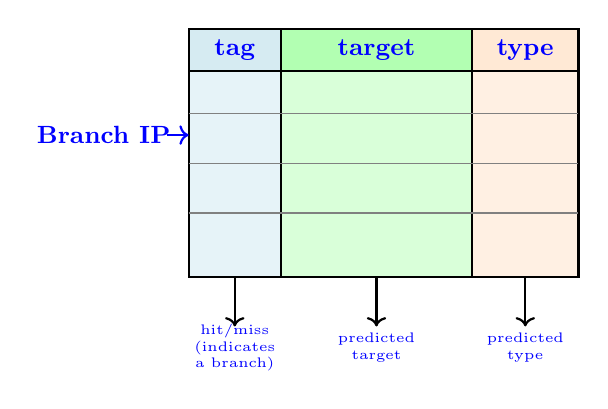
\begin{tikzpicture}[scale=0.9]
    % Define dimensions
    \def\tablewidth{5.5}
    \def\tableheight{3.5}
    \def\headerheight{0.6}
    \def\tagwidth{1.3}
    \def\targetwidth{2.7}
    \def\typewidth{1.5}
    
    % Draw the main table structure with colored columns
    % Tag column background
    \fill[lightblue!30] (0,0) rectangle (\tagwidth, -\tableheight);
    % Target column background  
    \fill[green!15] (\tagwidth,0) rectangle (\tagwidth+\targetwidth, -\tableheight);
    % Type column background
    \fill[peach!40] (\tagwidth+\targetwidth,0) rectangle (\tablewidth, -\tableheight);
    
    % Draw header row with stronger colors
    \fill[lightblue!50] (0,0) rectangle (\tagwidth, -\headerheight);
    \fill[green!30] (\tagwidth,0) rectangle (\tagwidth+\targetwidth, -\headerheight);
    \fill[peach!60] (\tagwidth+\targetwidth,0) rectangle (\tablewidth, -\headerheight);
    
    % Draw the table border
    \draw[thick, black] (0,0) rectangle (\tablewidth, -\tableheight);
    
    % Draw column dividers
    \draw[thick] (\tagwidth, 0) -- (\tagwidth, -\tableheight);
    \draw[thick] (\tagwidth+\targetwidth, 0) -- (\tagwidth+\targetwidth, -\tableheight);
    
    % Draw header separator
    \draw[thick] (0, -\headerheight) -- (\tablewidth, -\headerheight);
    
    % Add some row lines to show it's a table
    \foreach \y in {1.2, 1.9, 2.6} {
        \draw[gray, thin] (0, -\y) -- (\tablewidth, -\y);
    }
    
    % Header labels
    \node[myblue, font=\small\bfseries] at (\tagwidth/2, -\headerheight/2) {tag};
    \node[myblue, font=\small\bfseries] at (\tagwidth+\targetwidth/2, -\headerheight/2) {target};
    \node[myblue, font=\small\bfseries] at (\tagwidth+\targetwidth+\typewidth/2, -\headerheight/2) {type};
    
    % Branch IP label and arrow pointing to table
    \node[myblue, font=\small\bfseries] at (-1.2, -1.5) {Branch IP};
    \draw[->, thick, myblue] (-0.3, -1.5) -- (0, -1.5);
    
    % Output arrows and labels below the table
    \draw[->, thick] (\tagwidth/2, -\tableheight) -- (\tagwidth/2, -\tableheight-0.7);
    \node[align=center, font=\tiny, myblue] at (\tagwidth/2, -\tableheight-1.0) {hit/miss\\(indicates\\a branch)};
    
    \draw[->, thick] (\tagwidth+\targetwidth/2, -\tableheight) -- (\tagwidth+\targetwidth/2, -\tableheight-0.7);
    \node[align=center, font=\tiny, myblue] at (\tagwidth+\targetwidth/2, -\tableheight-1.0) {predicted\\target};
    
    \draw[->, thick] (\tagwidth+\targetwidth+\typewidth/2, -\tableheight) -- (\tagwidth+\targetwidth+\typewidth/2, -\tableheight-0.7);
    \node[align=center, font=\tiny, myblue] at (\tagwidth+\targetwidth+\typewidth/2, -\tableheight-1.0) {predicted\\type};
\end{tikzpicture}
\end{center}
\end{column}
\end{columns}

\end{frame}




\begin{frame}{The Target Array}
\begin{columns}[T,onlytextwidth]
  \begin{column}{0.63\textwidth}
    \begin{itemize}
      \item The TA is accessed using the branch address (branch IP)
      \begin{itemize}
        \item Implemented as an $n$-way set associative cache
      \end{itemize}

      \item The TA predicts the following
      \begin{itemize}
        \item Instruction is a branch
        \item Predicted target
        \item Branch type
        \begin{itemize}
          \item Conditional: jump to target if predict taken
          \item Unconditional direct: take target
          \item Unconditional indirect: if iTA hits, use its target
          \item Return: get target from Return Stack Buffer
        \end{itemize}
      \end{itemize}

      \item The TA is allocated/updated at Decode / EXE

      \item Tags are usually partial
      \begin{itemize}
        \item Trade-off space, can get false hits
        \item Few branches aliased to same entry
        \item No correctness, only performance
      \end{itemize}
    \end{itemize}
  \end{column}

  \begin{column}{0.37\textwidth}
    \centering
    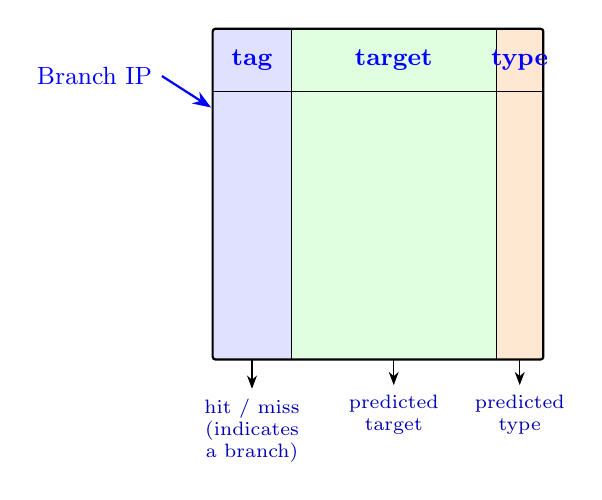
\begin{tikzpicture}[>=Stealth, node distance=2mm]
      % Sizes
      \def\W{4.2}   % total width
      \def\H{4.2}   % total height
      \def\tagw{1.0}
      \def\targetw{2.6}
      \def\typew{0.6}

      % Background column tints
      \fill[blue!12]   (0,-\H) rectangle (\tagw,0);
      \fill[green!12]  (\tagw,-\H) rectangle (\tagw+\targetw,0);
      \fill[orange!18] (\tagw+\targetw,-\H) rectangle (\W,0);

      % Outer box
      \draw[rounded corners=1pt, line width=0.8pt] (0,0) rectangle (\W,-\H);

      % Column dividers
      \draw (\tagw,0) -- (\tagw,-\H);
      \draw (\tagw+\targetw,0) -- (\tagw+\targetw,-\H);

      % Header separator
      \draw (0,-0.8) -- (\W,-0.8);

      % Header labels
      \node[font=\small\bfseries,blue]   at ($(0,0)!0.5!(\tagw,0)+(0,-0.4)$) {tag};
      \node[font=\small\bfseries,blue]   at ($(\tagw,0)!0.5!(\tagw+\targetw,0)+(0,-0.4)$) {target};
      \node[font=\small\bfseries,blue]   at ($(\tagw+\targetw,0)!0.5!(\W,0)+(0,-0.4)$) {type};

      % Branch IP input (left)
      \node[align=left, blue] (bp) at (-1.5,-0.6) {\small Branch IP};
      \draw[->,blue,thick] (bp.east) -- (-0.02,-1.0);

      % Bottom outputs
      \node[align=center, font=\scriptsize, blue!70!black] (hit) at (\tagw/2,-\H-0.9) {hit / miss\\(indicates\\a branch)};
      \draw[->] (\tagw/2,-\H) -- (hit.north);

      \node[align=center, font=\scriptsize, blue!70!black] (pt) at (\tagw+\targetw/2,-\H-0.7) {predicted\\target};
      \draw[->] (\tagw+\targetw/2,-\H) -- (pt.north);

      \node[align=center, font=\scriptsize, blue!70!black] (ty) at (\tagw+\targetw+\typew/2,-\H-0.7) {predicted\\type};
      \draw[->] (\tagw+\targetw+\typew/2,-\H) -- (ty.north);
    \end{tikzpicture}
  \end{column}
\end{columns}
\end{frame}


% Second Slide (previously first)
\begin{frame}
\frametitle{Bimodal Predictor (cont.)}
\label{frame:bimodal_predictor_cont}

\vspace{-0.2cm}

\begin{center}
\textcolor{myblue}{\textbf{2-bit-sat counter array}}
\end{center}

\vspace{0.2cm}

\begin{center}
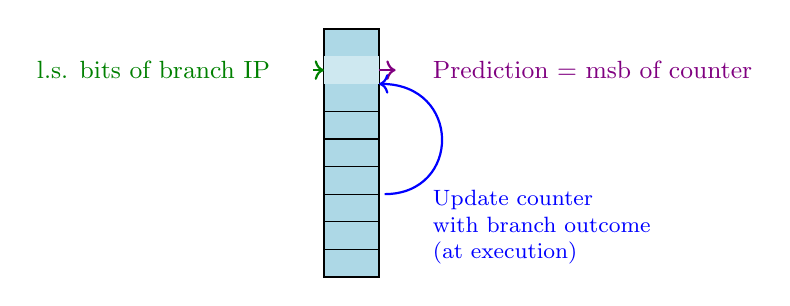
\begin{tikzpicture}[scale=0.7]
    % Draw the counter array
    \fill[lightblue] (0,0) rectangle (1,4.5);
    \draw[thick] (0,0) rectangle (1,4.5);
    
    % Draw array divisions
    \foreach \y in {0.5,1,1.5,2,2.5,3,3.5,4} {
        \draw (0,\y) -- (1,\y);
    }
    
    % Highlight the second cell from top (the one being accessed)
    \fill[lightblue!60] (0,3.5) rectangle (1,4);
    
    % Labels and arrows - pointing to second cell from top
    \node[mygreen,anchor=east,font=\small] at (-0.8,3.75) {l.s. bits of branch IP};
    \draw[->,thick,mygreen] (-0.2,3.75) -- (0,3.75);
    
    \node[mypurple,anchor=west,font=\small] at (1.8,3.75) {Prediction = msb of counter};
    \draw[->,thick,mypurple] (1,3.75) -- (1.3,3.75);
    
    % Curved arrow for update - starting low and curving up to second cell
    \draw[->,thick,myblue] (1.1,1.5) .. controls (2.5,1.5) and (2.5,3.5) .. (1,3.5);
    \node[myblue,align=left,anchor=west,font=\footnotesize] at (1.8,0.9) {Update counter\\with branch outcome\\(at execution)};
\end{tikzpicture}
\end{center}

\vspace{0.3cm}

\begin{itemize}
    \item[$\diamond$] \small\textbf{2-bit predictor avoids a double mistake in loops / glitches from the pattern}
\end{itemize}

\vspace{0.1cm}

{\footnotesize
\begin{tabular}{@{}ll@{}}
Branch Outcome & \texttt{0 0 0 0 0 1 0 0 0 0 0 1 0 0 0 0 0 1} \\
Prediction & \texttt{?~0 0 0 0 \textcolor{red}{0} 0 0 0 0 0 \textcolor{red}{0} 0 0 0 0 0 0} \\
\end{tabular}
}

\end{frame}


% Third Slide (previously second)
\begin{frame}
\frametitle{Bimodal (2-bit) Predictor}
\label{frame:bimodal_2bit}

%\vspace{-0.3cm}

% Indent bullet points and allow more horizontal space
\setlist[itemize]{left=0.5em, rightmargin=0.5em}
\begin{itemize}
    \item[$\diamond$] \textbf{A 2-bit counter avoids the double mistake in glitches}
    \begin{itemize}
        \item[$\circ$] Need "more evidence" to change prediction
    \end{itemize}
\end{itemize}

\vspace{-0.2cm}

\begin{center}
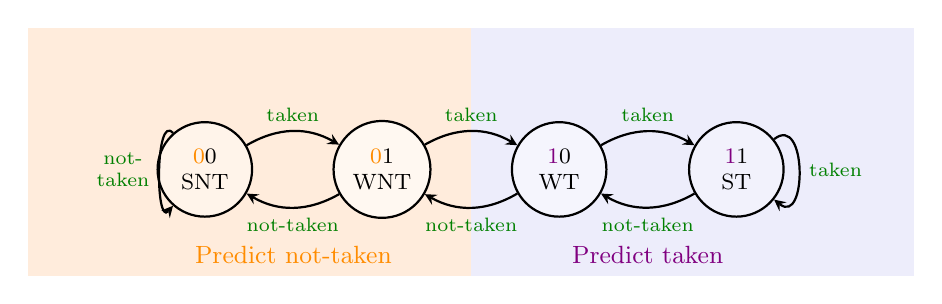
\begin{tikzpicture}[
    state/.style={circle,draw,thick,minimum size=1.2cm,font=\footnotesize,align=center},
    arrow/.style={->,>=stealth,thick},
    scale=0.9
]
    % Distinct background shades for prediction regions
    \begin{scope}[on background layer]
        \fill[peach!50] (-2.5,-1.5) rectangle (3.75,2); % Predict not-taken region
        \fill[lightpurple!70] (3.75,-1.5) rectangle (10,2); % Predict taken region, extended further right
    \end{scope}
    
    % States (LSB in black)
    \node[state,fill=peach!30] (SNT) at (0,0) {\textcolor{myorange}{0}\textcolor{black}{0}\\SNT};
    \node[state,fill=peach!20] (WNT) at (2.5,0) {\textcolor{myorange}{0}\textcolor{black}{1}\\WNT};
    \node[state,fill=lightpurple!40] (WT) at (5,0) {\textcolor{mypurple}{1}\textcolor{black}{0}\\WT};
    \node[state,fill=lightpurple!50] (ST) at (7.5,0) {\textcolor{mypurple}{1}\textcolor{black}{1}\\ST};
    
    % Self loop for SNT: from top left to bottom left, label on two lines
    \draw[arrow] (SNT) .. controls (-0.7,0.8) and (-0.7,-0.8) .. node[left,mygreen,font=\scriptsize,align=center] {not-\\taken} (SNT);
    % Self loop for ST: from top right to bottom right
    \draw[arrow] (ST) .. controls (8.5,0.8) and (8.5,-0.8) .. node[right,mygreen,font=\scriptsize,align=center] {taken} (ST);
    
    % Transitions between states
    \draw[arrow] (SNT) to[bend left=30] node[above,mygreen,font=\scriptsize] {taken} (WNT);
    \draw[arrow] (WNT) to[bend left=30] node[below,mygreen,font=\scriptsize] {not-taken} (SNT);
    
    \draw[arrow] (WNT) to[bend left=30] node[above,mygreen,font=\scriptsize] {taken} (WT);
    \draw[arrow] (WT) to[bend left=30] node[below,mygreen,font=\scriptsize] {not-taken} (WNT);
    
    \draw[arrow] (WT) to[bend left=30] node[above,mygreen,font=\scriptsize] {taken} (ST);
    \draw[arrow] (ST) to[bend left=30] node[below,mygreen,font=\scriptsize] {not-taken} (WT);
    
    % Prediction labels
    \node[myorange,font=\small] at (1.25,-1.2) {Predict not-taken};
    \node[mypurple,font=\small] at (6.25,-1.2) {Predict taken};
\end{tikzpicture}
\end{center}

\vspace{0.1cm}

\begin{itemize}
    \item[$\circ$] Initial state: weakly-taken (most branches are taken)
\end{itemize}

\begin{itemize}
    \item[$\diamond$] \textbf{Update (at execution)}
    \begin{itemize}
        \item[$\circ$] Branch was actually taken: increment counter (saturate at 11)
        \item[$\circ$] Branch was actually not-taken: decrement counter (saturate at 00)
    \end{itemize}
\end{itemize}

\begin{itemize}
    \item[$\diamond$] \textbf{Predict according to m.s.bit of counter (0=NT, 1=taken)}
    \item[$\diamond$] \textbf{Does not predict well branches with patterns like 010101...}
\end{itemize}

\end{frame}

\begin{frame}
\frametitle{Bimodal Predictor - example}
\label{frame:bimodal_example}

\begin{columns}[T]
\begin{column}{0.62\textwidth}

% Br1 prediction with tabular and vertical arrows
\begin{itemize}
\item[$\diamond$] \textbf{Br1 prediction}
\end{itemize}
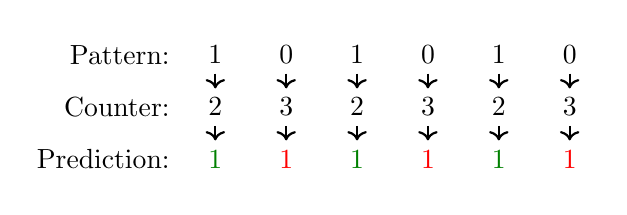
\begin{tikzpicture}[baseline=(current bounding box.center),every node/.style={anchor=base}]
    % Table for alignment
    \matrix[matrix of nodes,nodes={minimum width=0.5cm,anchor=center},column sep=0.4cm,row sep=0.2cm,ampersand replacement=\&] (m) {
        1 \& 0 \& 1 \& 0 \& 1 \& 0 \\
        2 \& 3 \& 2 \& 3 \& 2 \& 3 \\
        \textcolor{mygreen}{1} \& \textcolor{red}{1} \& \textcolor{mygreen}{1} \& \textcolor{red}{1} \& \textcolor{mygreen}{1} \& \textcolor{red}{1} \\
    };
    % Arrows from pattern to counter
    \foreach \i in {1,...,6} {
        \draw[->,thick] (m-1-\i.south) -- (m-2-\i.north);
        \draw[->,thick] (m-2-\i.south) -- (m-3-\i.north);
    }
    % Labels
    \node[left=0.2cm of m-1-1,align=right] {Pattern:};
    \node[left=0.2cm of m-2-1,align=right] {Counter:};
    \node[left=0.2cm of m-3-1,align=right] {Prediction:};
\end{tikzpicture}

\vspace{0.2cm}
% Br2 prediction with tabular and vertical arrows
\begin{itemize}
\item[$\diamond$] \textbf{Br2 prediction}
\end{itemize}
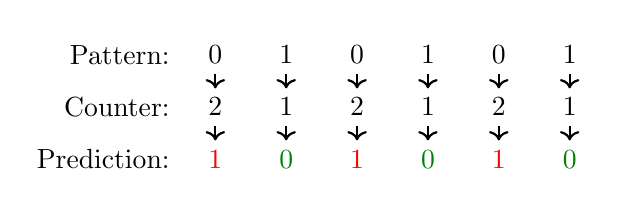
\begin{tikzpicture}[baseline=(current bounding box.center),every node/.style={anchor=base}]
    % Table for alignment
    \matrix[matrix of nodes,nodes={minimum width=0.5cm,anchor=center},column sep=0.4cm,row sep=0.2cm,ampersand replacement=\&] (m) {
        0 \& 1 \& 0 \& 1 \& 0 \& 1 \\
        2 \& 1 \& 2 \& 1 \& 2 \& 1 \\
        \textcolor{red}{1} \& \textcolor{mygreen}{0} \& \textcolor{red}{1} \& \textcolor{mygreen}{0} \& \textcolor{red}{1} \& \textcolor{mygreen}{0} \\
    };
    % Arrows from pattern to counter
    \foreach \i in {1,...,6} {
        \draw[->,thick] (m-1-\i.south) -- (m-2-\i.north);
        \draw[->,thick] (m-2-\i.south) -- (m-3-\i.north);
    }
    % Labels
    \node[left=0.2cm of m-1-1,align=right] {Pattern:};
    \node[left=0.2cm of m-2-1,align=right] {Counter:};
    \node[left=0.2cm of m-3-1,align=right] {Prediction:};
\end{tikzpicture}

\vspace{0.2cm}
% Br3 prediction with tabular and vertical arrows
\begin{itemize}
\item[$\diamond$] \textbf{Br3 prediction}
\end{itemize}
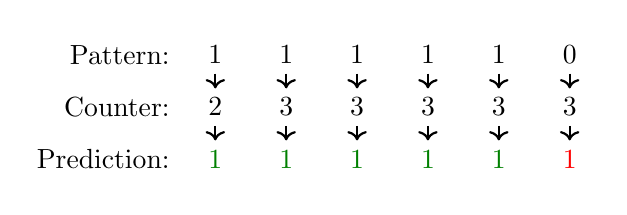
\begin{tikzpicture}[baseline=(current bounding box.center),every node/.style={anchor=base}]
    % Table for alignment
    \matrix[matrix of nodes,nodes={minimum width=0.5cm,anchor=center},column sep=0.4cm,row sep=0.2cm,ampersand replacement=\&] (m) {
        1 \& 1 \& 1 \& 1 \& 1 \& 0 \\
        2 \& 3 \& 3 \& 3 \& 3 \& 3 \\
        \textcolor{mygreen}{1} \& \textcolor{mygreen}{1} \& \textcolor{mygreen}{1} \& \textcolor{mygreen}{1} \& \textcolor{mygreen}{1} \& \textcolor{red}{1} \\
    };
    % Arrows from pattern to counter
    \foreach \i in {1,...,6} {
        \draw[->,thick] (m-1-\i.south) -- (m-2-\i.north);
        \draw[->,thick] (m-2-\i.south) -- (m-3-\i.north);
    }
    % Labels
    \node[left=0.2cm of m-1-1,align=right] {Pattern:};
    \node[left=0.2cm of m-2-1,align=right] {Counter:};
    \node[left=0.2cm of m-3-1,align=right] {Prediction:};
\end{tikzpicture}

\end{column}

\begin{column}{0.38\textwidth}
\vspace{1cm}
\begin{tcolorbox}[
    colback=lightblue!10,
    colframe=myblue,
    boxrule=1pt,
    arc=2mm,
    left=3mm,
    right=3mm,
    top=3mm,
    bottom=3mm,
    fontupper=\footnotesize\ttfamily
]
\textbf{\normalfont\small Code:}

\vspace{0.2cm}
int n = 6;

\vspace{0.2cm}
Loop: \hspace{0.3cm} ....

\vspace{0.2cm}
br1: if (n\%2) \{ ... \}

\vspace{0.2cm}
br2: if ((n+1)\%2) \{ ... \}

\vspace{0.3cm}
\hspace{0.5cm} n{-}{-};

\vspace{0.2cm}
br3: JNZ n, Loop
\end{tcolorbox}
\end{column}
\end{columns}

\end{frame}


\end{document}